\documentclass{ximera}

\title{Practice for Slope Fields}

%\auor{Matthew Charnley and Jason Nowell}
\usepackage[margin=1.5cm]{geometry}
\usepackage{indentfirst}
\usepackage{sagetex}
\usepackage{lipsum}
\usepackage{amsmath}
\usepackage{mathrsfs}


%%% Random packages added without verifying what they are really doing - just to get initial compile to work.
\usepackage{tcolorbox}
\usepackage{hypcap}
\usepackage{booktabs}%% To get \toprule,\midrule,\bottomrule etc.
\usepackage{nicefrac}
\usepackage{caption}
\usepackage{units}

% This is my modified wrapfig that doesn't use intextsep
\usepackage{mywrapfig}
\usepackage{import}



%%% End to random added packages.


\graphicspath{
    {./figures/}
    {./../figures/}
    {./../../figures/}
}
\renewcommand{\log}{\ln}%%%%
\DeclareMathOperator{\arcsec}{arcsec}
%% New commands


%%%%%%%%%%%%%%%%%%%%
% New Conditionals %
%%%%%%%%%%%%%%%%%%%%


% referencing
\makeatletter
    \DeclareRobustCommand{\myvref}[2]{%
      \leavevmode%
      \begingroup
        \let\T@pageref\@pagerefstar
        \hyperref[{#2}]{%
	  #1~\ref*{#2}%
        }%
        \vpageref[\unskip]{#2}%
      \endgroup
    }%

    \DeclareRobustCommand{\myref}[2]{%
      \leavevmode%
      \begingroup
        \let\T@pageref\@pagerefstar
        \hyperref[{#2}]{%
	  #1~\ref*{#2}%
        }%
      \endgroup
    }%
\makeatother

\newcommand{\figurevref}[1]{\myvref{Figure}{#1}}
\newcommand{\figureref}[1]{\myref{Figure}{#1}}
\newcommand{\tablevref}[1]{\myvref{Table}{#1}}
\newcommand{\tableref}[1]{\myref{Table}{#1}}
\newcommand{\chapterref}[1]{\myref{chapter}{#1}}
\newcommand{\Chapterref}[1]{\myref{Chapter}{#1}}
\newcommand{\appendixref}[1]{\myref{appendix}{#1}}
\newcommand{\Appendixref}[1]{\myref{Appendix}{#1}}
\newcommand{\sectionref}[1]{\myref{\S}{#1}}
\newcommand{\subsectionref}[1]{\myref{subsection}{#1}}
\newcommand{\subsectionvref}[1]{\myvref{subsection}{#1}}
\newcommand{\exercisevref}[1]{\myvref{Exercise}{#1}}
\newcommand{\exerciseref}[1]{\myref{Exercise}{#1}}
\newcommand{\examplevref}[1]{\myvref{Example}{#1}}
\newcommand{\exampleref}[1]{\myref{Example}{#1}}
\newcommand{\thmvref}[1]{\myvref{Theorem}{#1}}
\newcommand{\thmref}[1]{\myref{Theorem}{#1}}


\renewcommand{\exampleref}[1]{ {\color{red} \bfseries Normally a reference to a previous example goes here.}}
\renewcommand{\figurevref}[1]{ {\color{red} \bfseries Normally a reference to a previous figure goes here.}}
\renewcommand{\tablevref}[1]{ {\color{red} \bfseries Normally a reference to a previous table goes here.}}
\renewcommand{\Appendixref}[1]{ {\color{red} \bfseries Normally a reference to an Appendix goes here.}}
\renewcommand{\exercisevref}[1]{ {\color{red} \bfseries Normally a reference to a previous exercise goes here.}}



\newcommand{\R}{\mathbb{R}}

%% Example Solution Env.
\def\beginSolclaim{\par\addvspace{\medskipamount}\noindent\hbox{\bf Solution:}\hspace{0.5em}\ignorespaces}
\def\endSolclaim{\par\addvspace{-1em}\hfill\rule{1em}{0.4pt}\hspace{-0.4pt}\rule{0.4pt}{1em}\par\addvspace{\medskipamount}}
\newenvironment{exampleSol}[1][]{\beginSolclaim}{\endSolclaim}

%% General figure formating from original book.
\newcommand{\mybeginframe}{%
\begin{tcolorbox}[colback=white,colframe=lightgray,left=5pt,right=5pt]%
}
\newcommand{\myendframe}{%
\end{tcolorbox}%
}

%%% Eventually return and fix this to make matlab code work correctly.
%% Define the matlab environment as another code environment
%\newenvironment{matlab}
%{% Begin Environment Code
%{ \centering \bfseries Matlab Code }
%\begin{code}
%}% End of Begin Environment Code
%{% Start of End Environment Code
%\end{code}
%}% End of End Environment Code


% this one should have a caption, first argument is the size
\newenvironment{mywrapfig}[2][]{
 \wrapfigure[#1]{r}{#2}
 \mybeginframe
 \centering
}{%
 \myendframe
 \endwrapfigure
}

% this one has no caption, first argument is size,
% the second argument is a larger size used for HTML (ignored by latex)
\newenvironment{mywrapfigsimp}[3][]{%
 \wrapfigure[#1]{r}{#2}%
 \centering%
}{%
 \endwrapfigure%
}
\newenvironment{myfig}
    {%
    \begin{figure}[h!t]
        \mybeginframe%
        \centering%
    }
    {%
        \myendframe
    \end{figure}%
    }


% graphics include
\newcommand{\diffyincludegraphics}[3]{\includegraphics[#1]{#3}}
\newcommand{\myincludegraphics}[3]{\includegraphics[#1]{#3}}
\newcommand{\inputpdft}[1]{\subimport*{../figures/}{#1.pdf_t}}


%% Not sure what these even do? They don't seem to actually work... fun!
%\newcommand{\mybxbg}[1]{\tcboxmath[colback=white,colframe=black,boxrule=0.5pt,top=1.5pt,bottom=1.5pt]{#1}}
%\newcommand{\mybxsm}[1]{\tcboxmath[colback=white,colframe=black,boxrule=0.5pt,left=0pt,right=0pt,top=0pt,bottom=0pt]{#1}}
\newcommand{\mybxsm}[1]{#1}
\newcommand{\mybxbg}[1]{#1}

%%% Something about tasks for practice/hw?
\usepackage{tasks}
\usepackage{footnote}
\makesavenoteenv{tasks}


%% For pdf only?
\newcommand{\diffypdfversion}[1]{#1}


%% Kill ``cite'' and go back later to fix it.
\renewcommand{\cite}[1]{}


%% Currently we can't really use index or its derivatives. So we are gonna kill them off.
\renewcommand{\index}[1]{}
\newcommand{\myindex}[1]{#1}







\begin{document}
\begin{abstract}
    Why?
\end{abstract}
\maketitle

\begin{exercise}
    Sketch slope field for $y'=e^{x-y}$.  How do the solutions behave as $x$ grows?  Can you guess a particular solution by looking at the slope field?
\end{exercise}
%\comboSol
%{%
%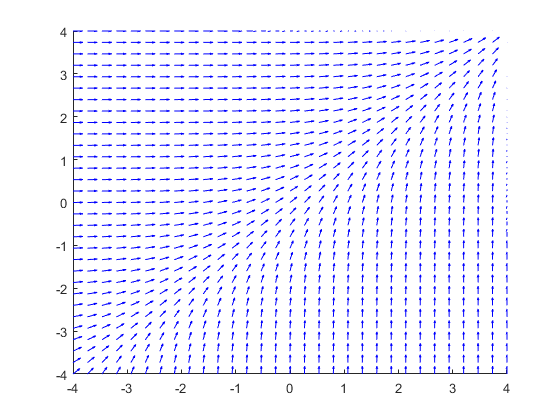
\includegraphics[width=2in]{slopefieldexpxmy.png}
%
%$y=x$ is a solution.
%}

\begin{exercise}%
    Sketch the slope field of $y'=y^3$.  Can you visually find the solution that satisfies $y(0)=0$?
\end{exercise}
%\exsol{%
%\\[6pt]
%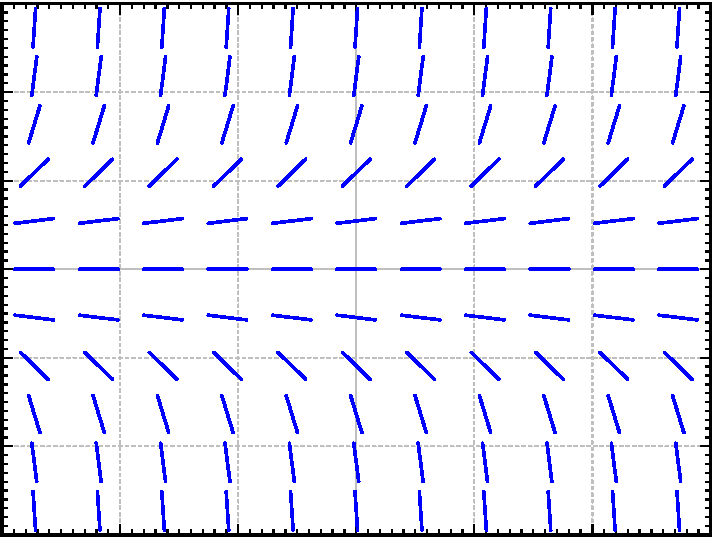
\includegraphics[width=2in]{yprimey3slope}
%\\
%$y=0$ is a solution such that $y(0)=0$.
%}


\begin{exercise}
    Sketch slope field for $y'=x^2$.
\end{exercise}
%\comboSol
%{%
%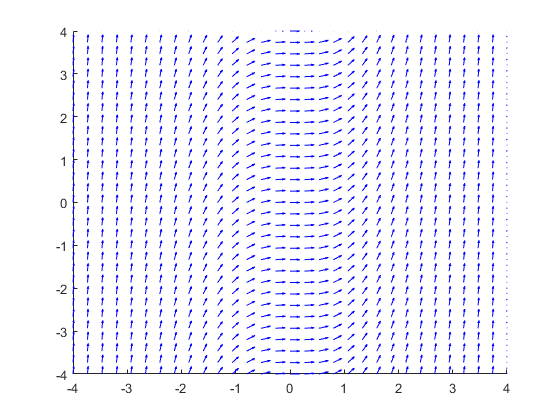
\includegraphics[width=2in]{slopefieldx2.png}
%}

\begin{exercise}
    Sketch slope field for $y'=y^2$.
\end{exercise}
%\comboSol
%{%
%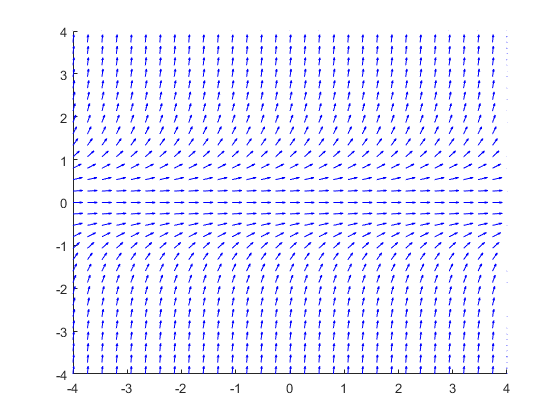
\includegraphics[width=2in]{slopefieldy2.png}
%}

\begin{exercise}
    For each of the following differential equations, sketch out a slope field on $-3 < x < 3$ and $-3 < y < 3$ and determine the overall behavior of the solutions to the equation as $t \rightarrow \infty$. If this fact depends on the value of the solution at $t=0$, explain how it changes.
    \begin{tasks}(4)
        \task $\displaystyle \frac{dy}{dx} = 3 - 2y$
        \task $\displaystyle \frac{dy}{dx} = 1 + y$
        \task $\displaystyle \frac{dy}{dx} = y - 1$
        \task $\displaystyle \frac{dy}{dx} = -2 - y$
    \end{tasks}
\end{exercise}
%\comboSol
%{%
%a)~\parbox[c]{1.2in}{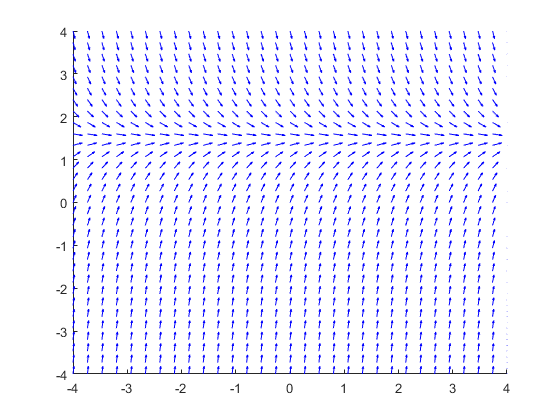
\includegraphics[width=1.2in]{slopefield3m2y.png}} \quad b)~\parbox[c]{1.2in}{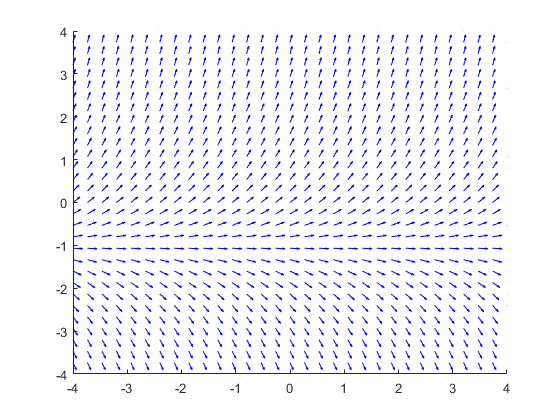
\includegraphics[width=1.2in]{slopefield1py.png}} \quad c)~\parbox[c]{1.2in}{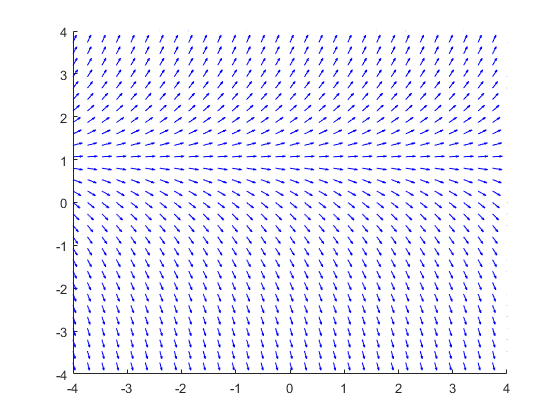
\includegraphics[width=1.2in]{slopefieldym1.png}} \quad d)~\parbox[c]{1.2in}{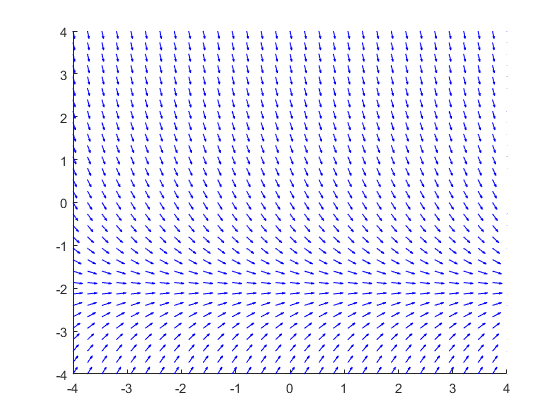
\includegraphics[width=1.2in]{slopefieldm2my.png}}
%
%a)~Solutions tend to $3/2$.
%b)~Solutions go to $\infty$ if $y(0) > -1$, goes to $-\infty$ is $y(0) < -1$. Constant if $y(0) = -1$. 
%c)~Solutions go to $\infty$ if $y(0) > 1$, goes to $-\infty$ is $y(0) < 1$. Constant if $y(0) = 1$. 
%d)~Solutions tend to $-2$.
%}

\begin{exercise}
    Which of the following slope fields corresponds to the differential equation $\frac{dy}{dt} = t(y-1)$. Explain your reasoning.
    \begin{tasks}(3)
        \task \parbox[c]{1.75in}{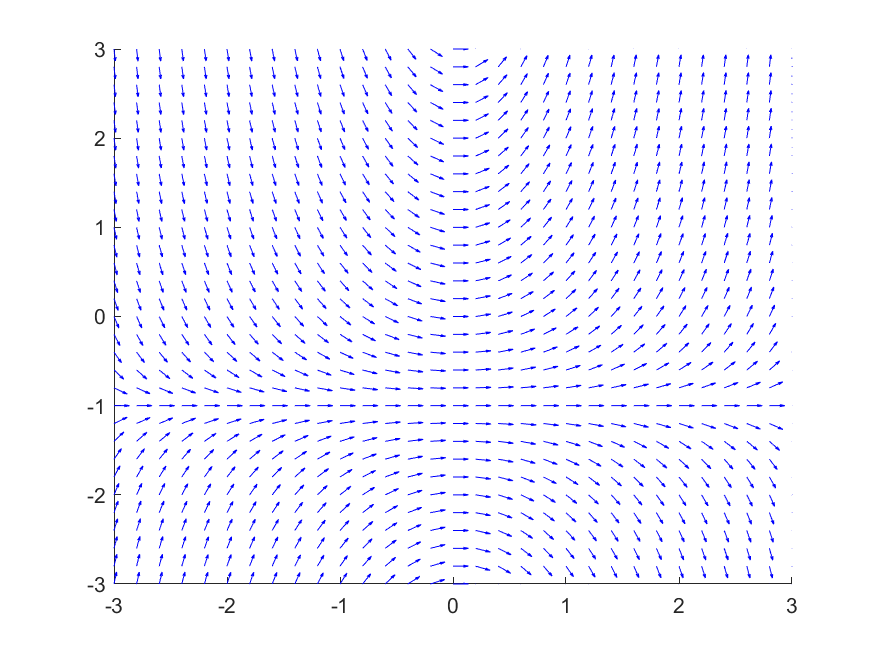
\includegraphics[width=1.75in]{yprimetyp1slope}}
        \task \parbox[c]{1.75in}{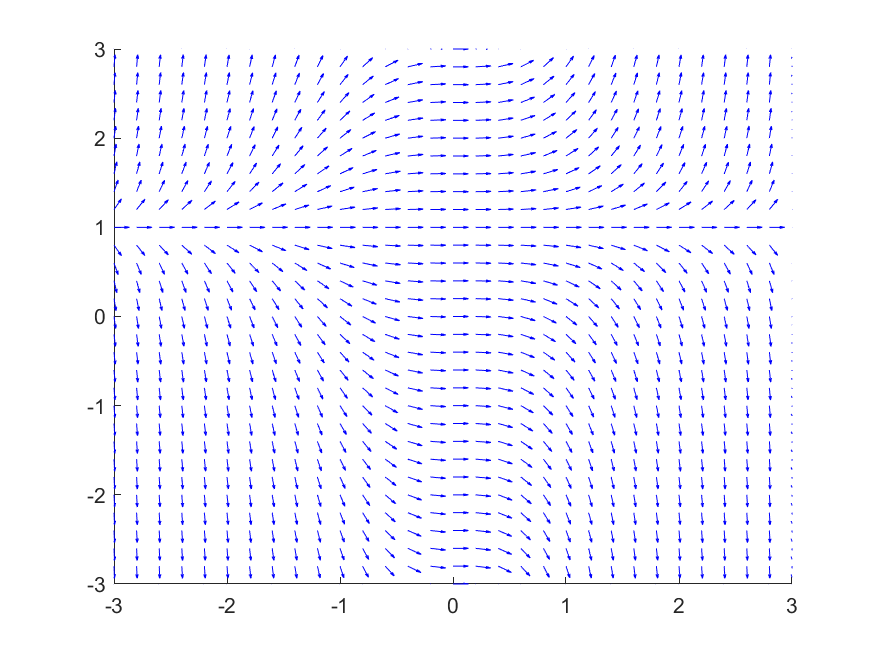
\includegraphics[width=1.75in]{yprimetsqym1slope}}
        \task \parbox[c]{1.75in}{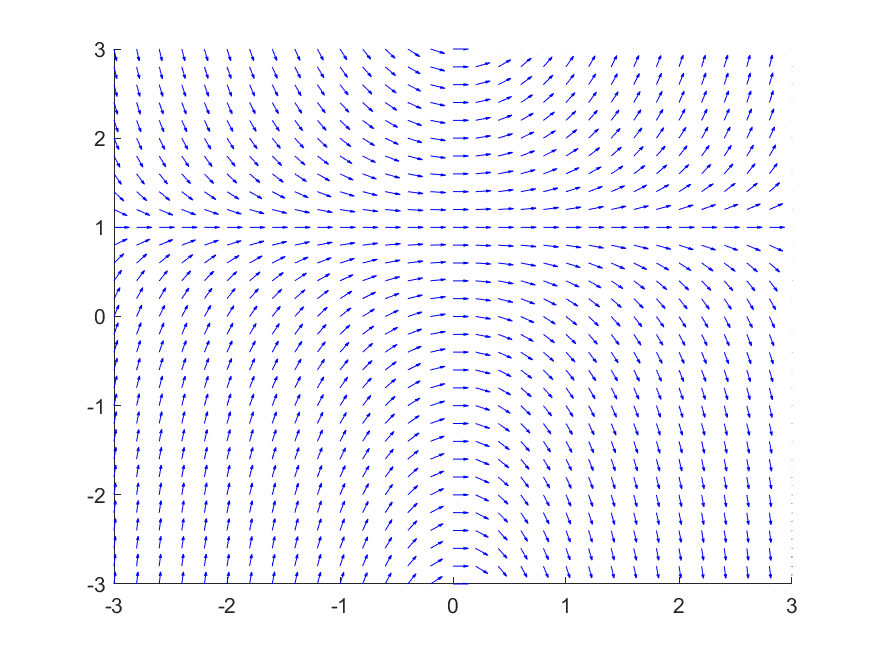
\includegraphics[width=1.75in]{yprimetym1slope}}
    \end{tasks}
\end{exercise}
%\comboSol
%{%
%b)
%}

\begin{exercise}
    Which of the following slope fields corresponds to the differential equation $\frac{dy}{dt} = (2-t)(y^2 - 9)$. Explain your reasoning.
    \begin{tasks}(3)
        \task \parbox[c]{1.75in}{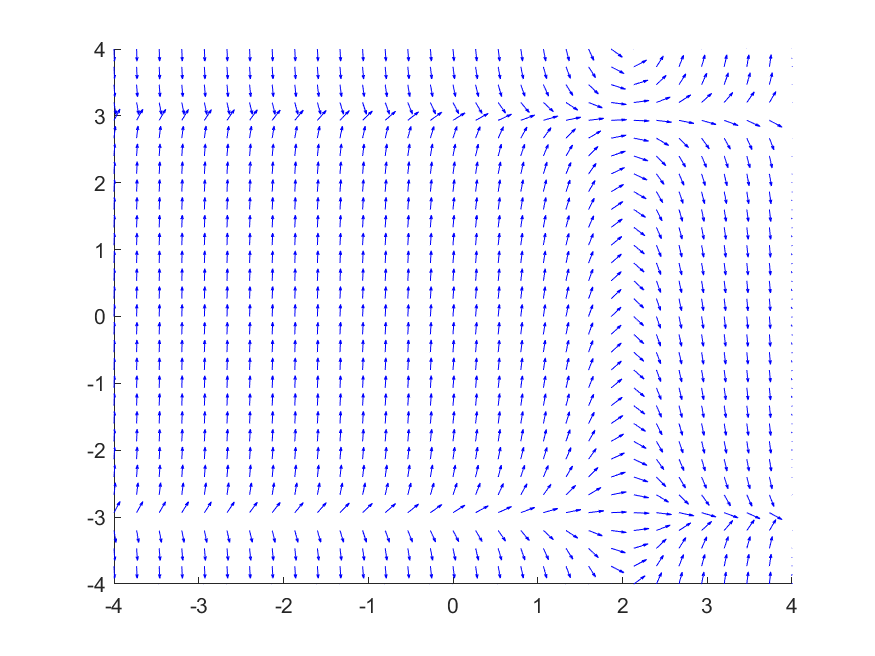
\includegraphics[width=1.75in]{yprimetm2ysqm9slope}}
        \task \parbox[c]{1.75in}{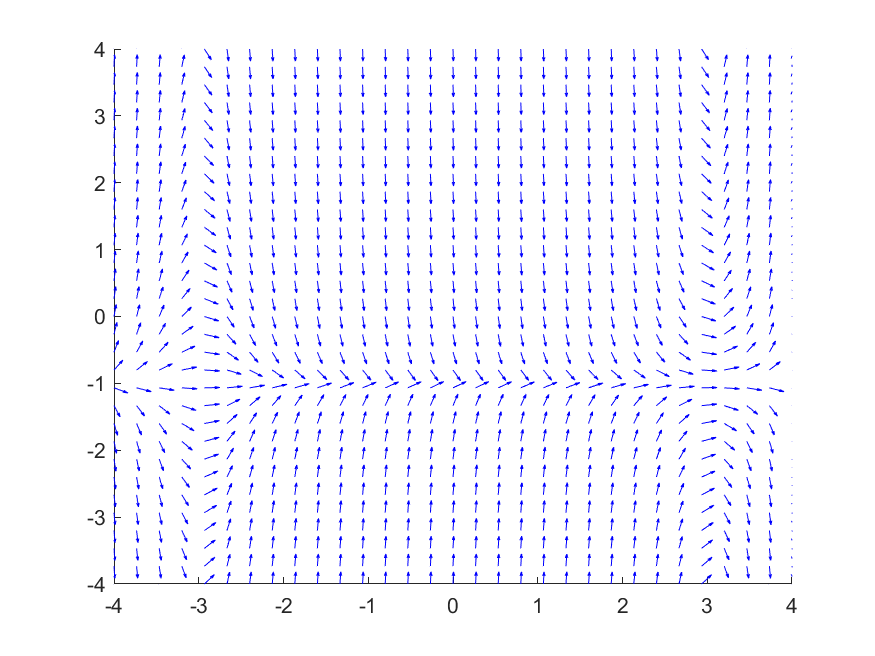
\includegraphics[width=1.75in]{yprimeyp1tsqm9slope}}
        \task \parbox[c]{1.75in}{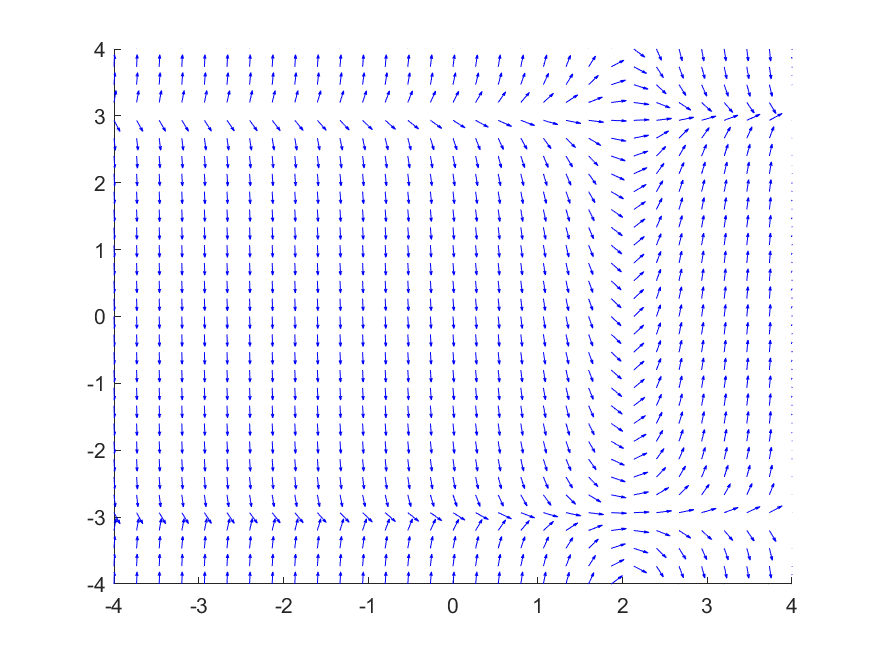
\includegraphics[width=1.75in]{yprime2mtysqm9slope}}
    \end{tasks}
\end{exercise}
%\comboSol
%{%
%c)
%}


\begin{exercise}
    Match equations $y'=1-x$, $y'=x-2y$, $y' = x(1-y)$ to slope fields. Justify.
    \begin{tasks}(3)
        \task \parbox[c]{1.75in}{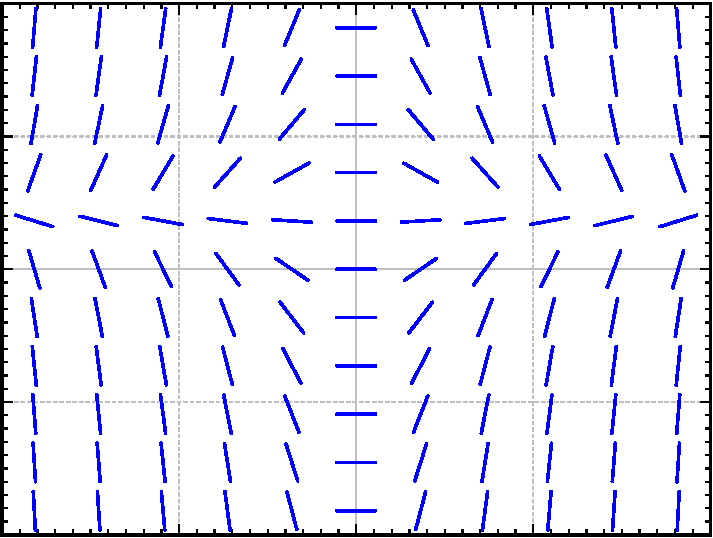
\includegraphics[width=1.75in]{yprimex1minusyslope}}
        \task \parbox[c]{1.75in}{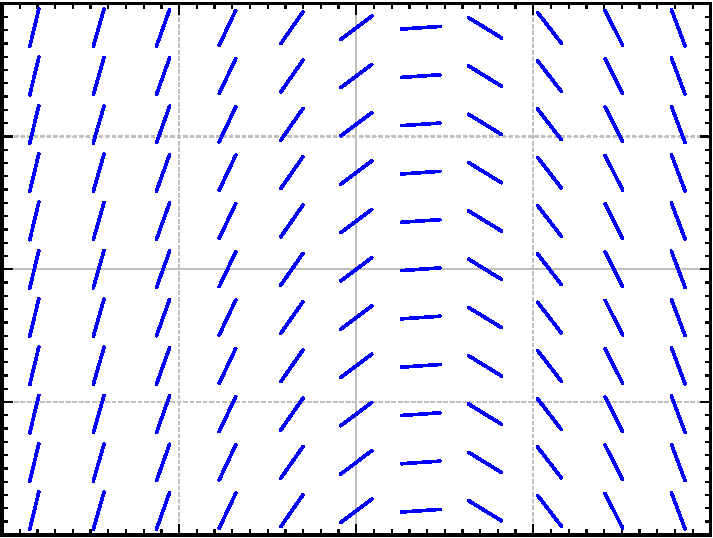
\includegraphics[width=1.75in]{yprime1minusxslope}}
        \task \parbox[c]{1.75in}{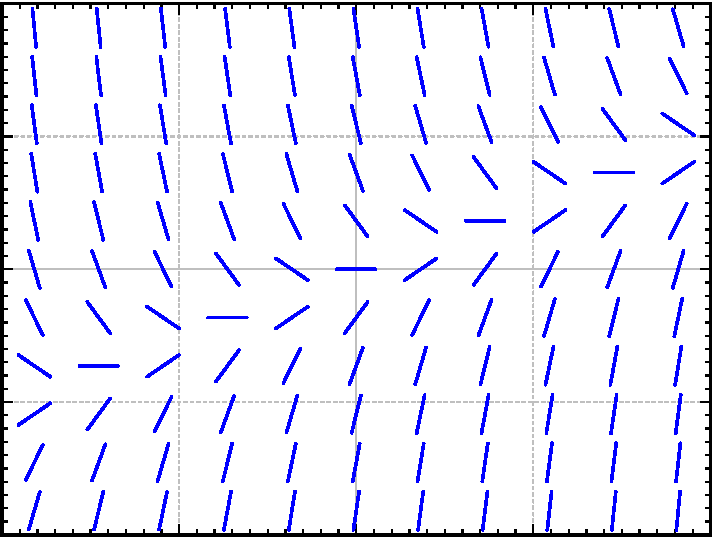
\includegraphics[width=1.75in]{yprimexminus2yslope}}
    \end{tasks}
\end{exercise}
%\comboSol
%{%
%a)~$y' = x(1-y)$ \quad b)~$y' = 1-x$ \quad c)~$y'=x-2y$
%}


\begin{exercise}%
    Match equations $y'=\sin x$, $y'=\cos y$, $y' = y\cos(x)$ to slope fields. Justify.
    \begin{tasks}(3)
        \task \parbox[c]{1.75in}{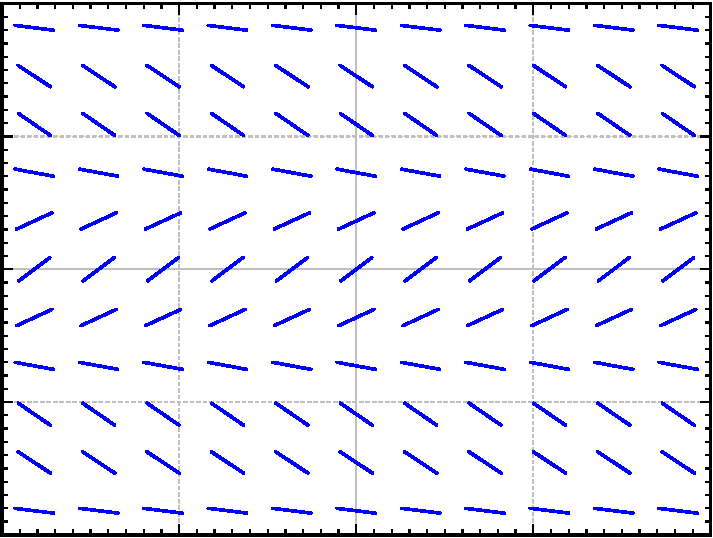
\includegraphics[width=1.75in]{yprimecosyslope}}
        \task \parbox[c]{1.75in}{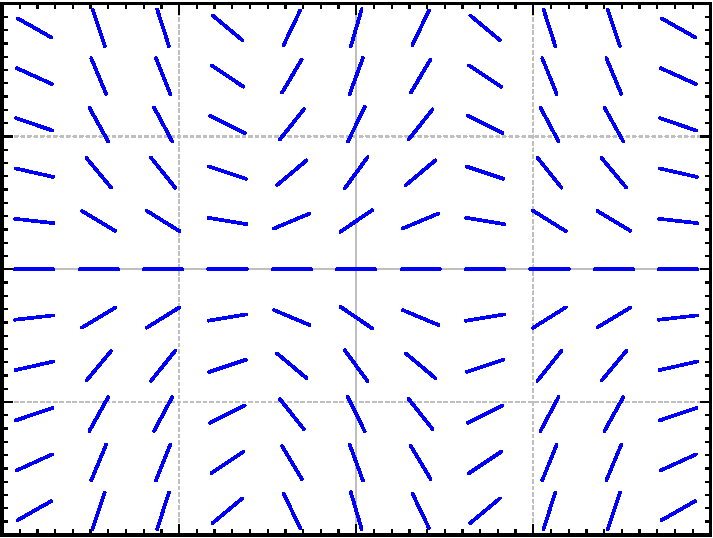
\includegraphics[width=1.75in]{yprimecosxyslope}}
        \task \parbox[c]{1.75in}{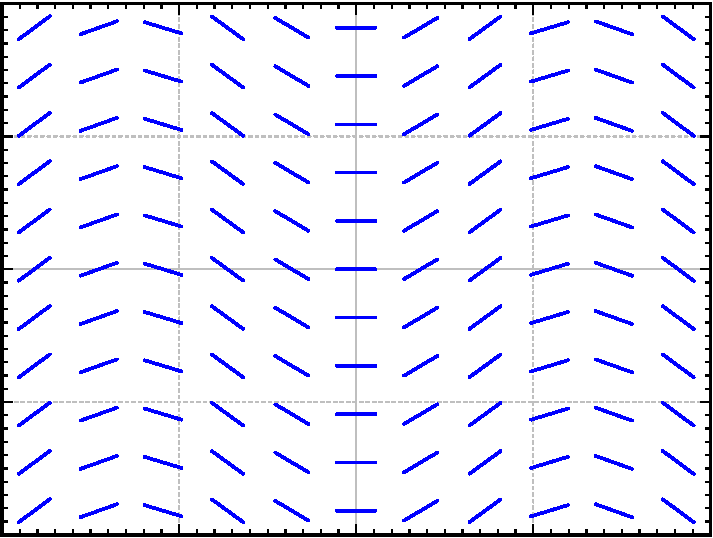
\includegraphics[width=1.75in]{yprimesinxslope}}
    \end{tasks}
\end{exercise}
%\exsol{%
%a) $y'=\cos y$, \quad
%b) $y' = y\cos(x)$, \quad
%c) $y'=\sin x$. \quad
%Justification left to reader.
%}

\begin{exercise}
    Match equations $y'=y(y-2)$, $y'=y-1$, $y' = y(2-y)$ to slope fields. Justify.
    \begin{tasks}(3)
        \task \parbox[c]{1.75in}{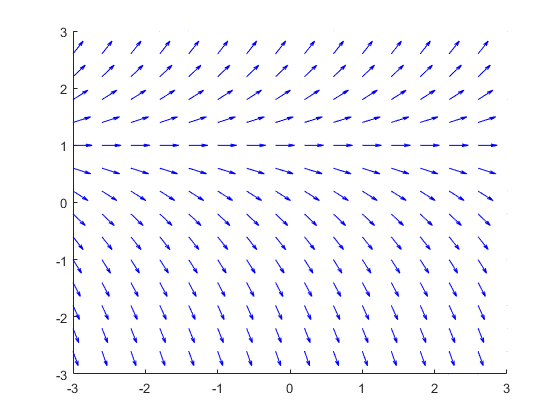
\includegraphics[width=2in]{quivym1}}
        \task \parbox[c]{1.75in}{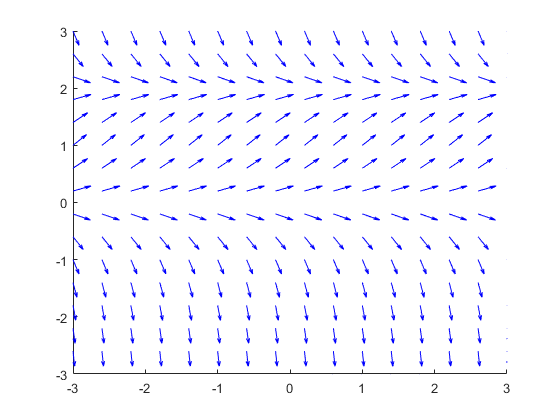
\includegraphics[width=2in]{quivy2my}}
        \task \parbox[c]{1.75in}{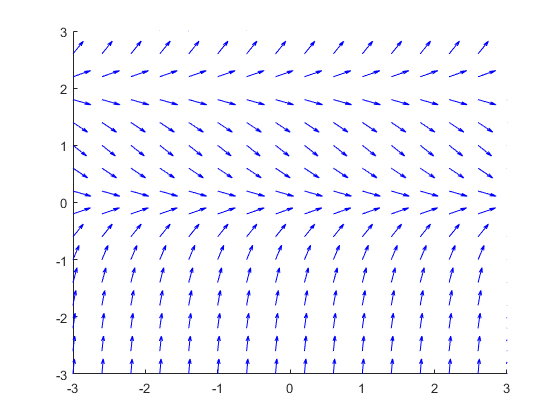
\includegraphics[width=2in]{quivyym2}}
    \end{tasks}
\end{exercise}
%\comboSol
%{%
%a)~$y'=y-1$\quad b)~$y'=y(2-y)$\quad c)~$y'=y(y-2)$
%}

\begin{exercise}
    Match equations $y'=t(y^2 + 1)$, $y'=t(y^2 - 1)$, $y' = t^2(y^2 - 1)$ to slope fields. Justify.
    \begin{tasks}(3)
        \task \parbox[c]{1.75in}{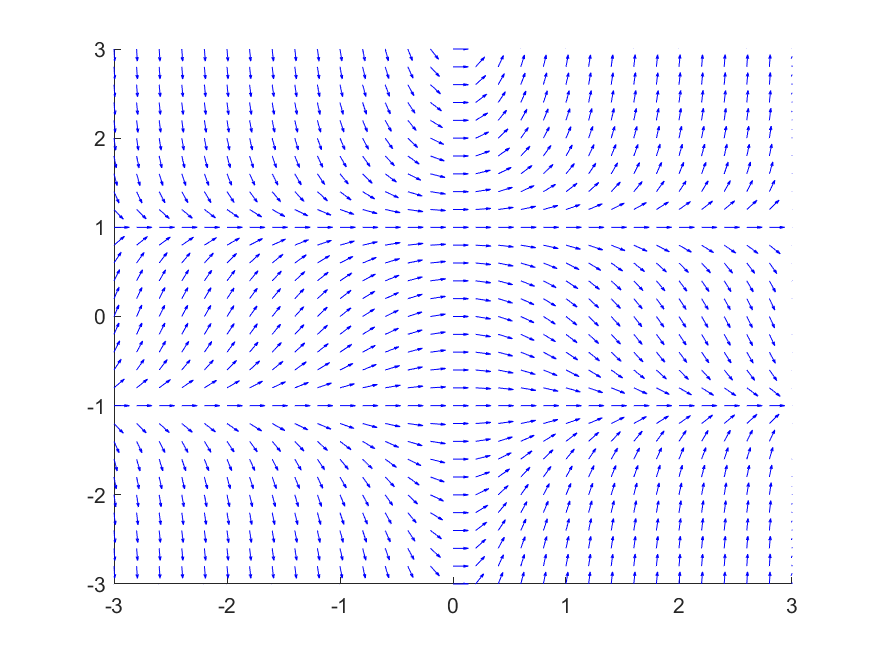
\includegraphics[width=2in]{yprimetysqm1slope}}
        \task \parbox[c]{1.75in}{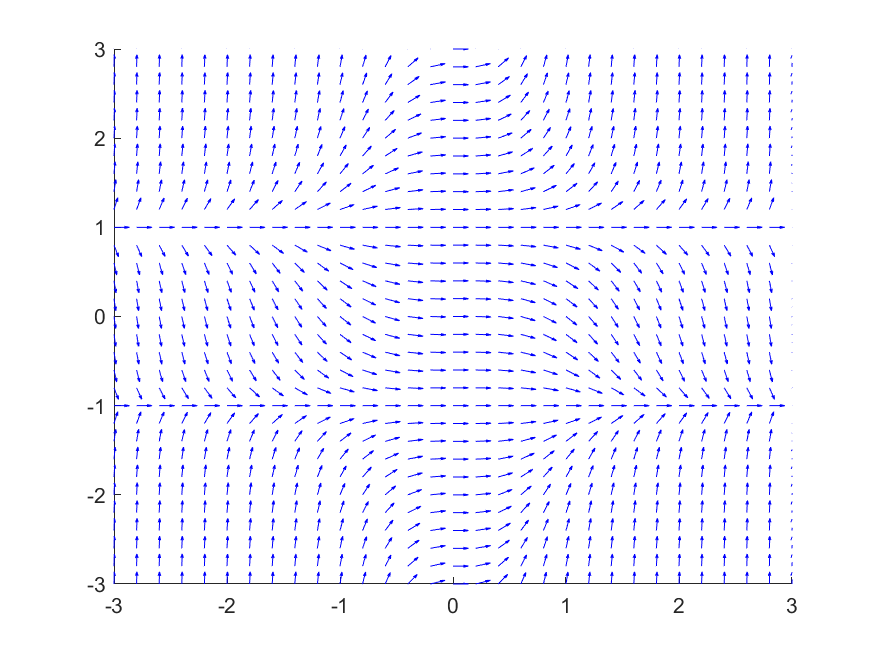
\includegraphics[width=2in]{yprimetsqysqm1slope}}
        \task \parbox[c]{1.75in}{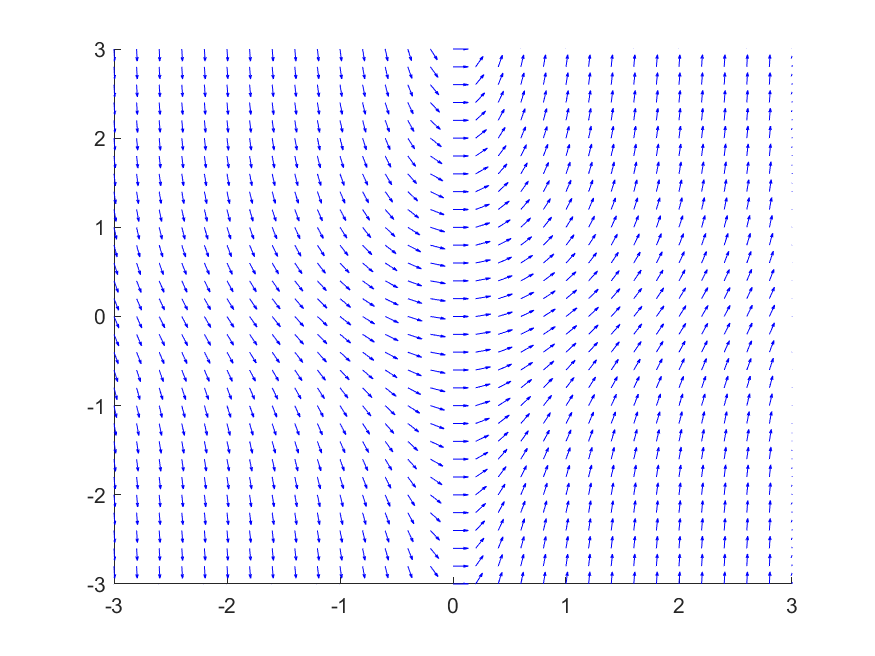
\includegraphics[width=2in]{yprimetysqp1slope}}
    \end{tasks}
\end{exercise}
%\comboSol
%{%
%a)~$y'=t(y^2 -1)$ \quad b)~$y'=t^2(y^2 - 1)$ \quad c)~$y'=t(y^2 + 1)$
%}

\begin{exercise}\label{ex:3myyp2}
    The slope field for the differential equation $y' = (3-y)(y+2)$ is below.  If we find the solution to this differential equation with initial condition, $y(0) = 1$, what will happen to the solution as $t \rightarrow \infty$? Use the slope field and your knowledge of the equation to determine the long-time behavior of this solution.
\end{exercise}
%\comboSol
%{%
%Tends to 3
%}

\begin{exercise}\label{ex:tm2yp4ym3}
    The slope field for the differential equation $y' = (t-2)(y+4)(y-3)$ is below. If we find the solution to this differential equation with initial condition, $y(0) = 1$, what will happen to the solution as $t \rightarrow \infty$? Use the slope field and your knowledge of the equation to determine the long-time behavior of this solution.
\end{exercise}
%\comboSol
%{%
%Tends to -4
%}

\begin{exercise}\label{ex:yp1yp4}
    The slope field for the differential equation $y' = (y+1)(y+4)$ is below. If we find the solution to this differential equation with initial condition, $y(0) = 1$, what will happen to the solution as $t \rightarrow \infty$? Use the slope field and your knowledge of the equation to determine the long-time behavior of this solution.
\end{exercise}
%\comboSol
%{%
%Goes to $\infty$. Will not exist for all positive $t$ values.
%}

\begin{minipage}{0.32\textwidth}
    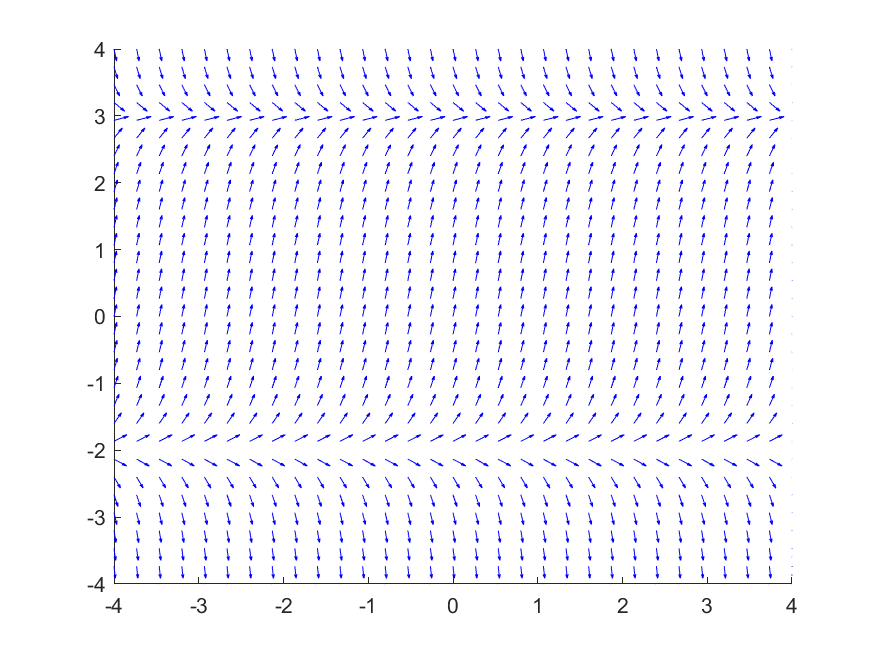
\includegraphics[width=\textwidth]{yprime3myyp2slope}
    \captionof{figure}{\exerciseref{ex:3myyp2}}
\end{minipage}%
\begin{minipage}{0.32\textwidth}
    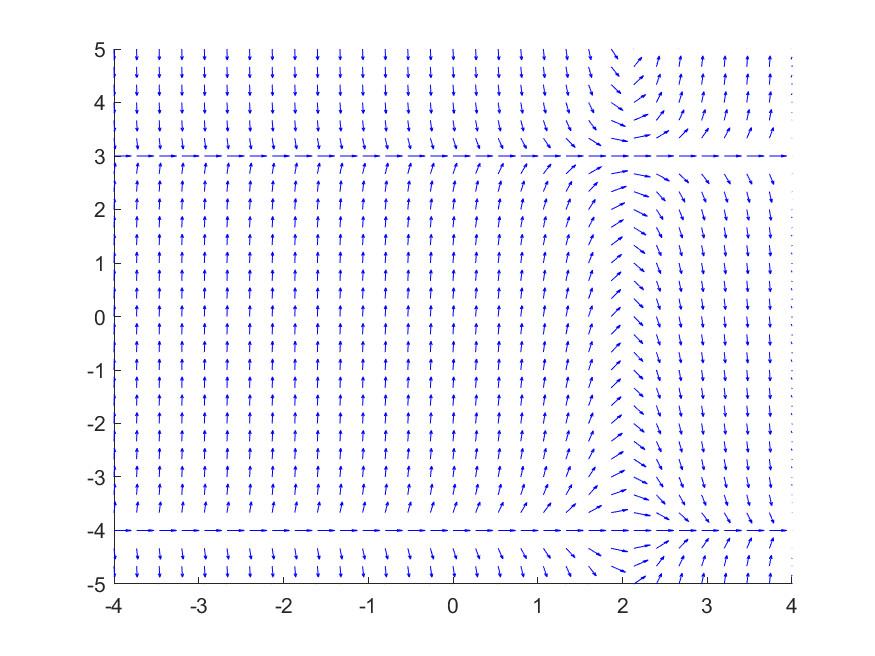
\includegraphics[width=\textwidth]{yprimetm2yp4ym3slope}
    \captionof{figure}{\exerciseref{ex:tm2yp4ym3}}
\end{minipage}%
\begin{minipage}{0.32\textwidth}
    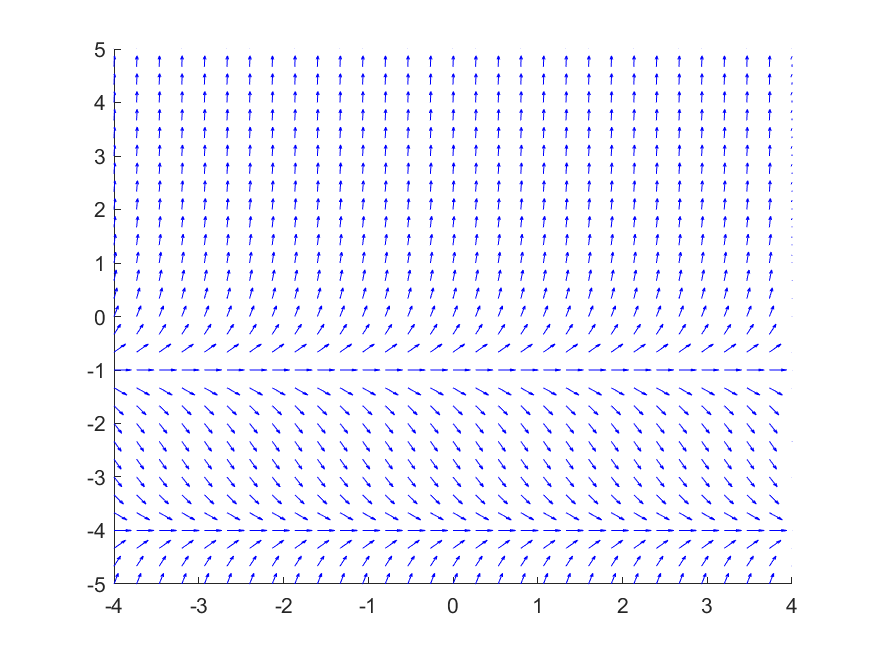
\includegraphics[width=\textwidth]{yprimeyp1yp4slope}
    \captionof{figure}{\exerciseref{ex:yp1yp4}}
\end{minipage}

\begin{exercise}[challenging]
    Take $y' = f(x,y)$, $y(0) = 0$, where $f(x,y) > 1$ for all $x$ and $y$.  If the solution exists for all $x$, can you say what happens to $y(x)$ as $x$ goes to positive infinity?  Explain.
\end{exercise}
%\comboSol
%{%
%Yes, it will go to $\infty$.
%}

\begin{exercise}
    Suppose $y' = f(x,y)$.  What will the slope field look like, explain and sketch an example, if you know the following about $f(x,y)$:
    \begin{tasks}(2)
        \task $f$ does not depend on $y$.
        \task $f$ does not depend on $x$.
        \task $f(t,t) = 0$ for any number $t$.
        \task $f(x,0) = 0$ and $f(x,1) = 1$ for all $x$.
    \end{tasks}
\end{exercise}
%\comboSol
%{%
%a)~Slopes are independent of $y$. On a vertical line, the slopes are all the same. \\
%b)~Slopes are independent of $x$. Horizontal invariance. \\
%c)~Horizontal tangents along the line $y=x$.\\
%d)~Horizontal tangents along the $x$-axis, so $x=0$ is a solution. Slope $1$ along $y=1$. 
%}

\begin{exercise}
    Describe what each of the following facts about the function $f(x,y)$ tells you about the slope field for the differential equation $y' = f(x,y)$.
    \begin{tasks}
        \task $f(2,y) = 0$ for all $y$
        \task $f(x,-x) = 0$ for all $x$
        \task $f(x,x) = 1$ for all $x$
        \task $f(x, -1) = 0$ for all $x$
    \end{tasks}
\end{exercise}
%\comboSol
%{%
%a)~Horizontal tangents along $x=2$.\\
%b)~Horizontal tangents along the line $y=-x$.\\
%c)~Slope one along the line $y=x$. Also $y=x$ is a solution.\\
%d)~Horizontal tangents along the line $y=-1$.
%}

%\setcounter{exercise}{100}



\end{document}